%!TEX root = ../main.tex
\setcounter{chapter}{2}
\chapter{Dynamic programming}
	In this exercise, we tackle the trajectory planning problem through a dynamic-programming-based approach.
	Trajectory planning refers to the task of planning, in a certain temporary horizon, the sequence of control needed to reach a certain control objective in an optimal way. 
	This is an important problem for autonomous vehicles because they must make decisions considering specific navigation requirements such as avoiding obstacles, while staying within their own lane. 
	\par
	%
	In particular, the problem is often solved in four steps as follows:
	\begin{enumerate}
		\item a certain cost function is defined related to the control objectives,
		\item the current state of the vehicle as well as the set of valid control actions are used to generate a graph representing the feasible trajectories that can be followed by the vehicle,
		\item each trajectory is evaluated according to the cost function,
		\item the best trajectory out of the generated ones is chosen.
	\end{enumerate} 
	%
	In this exercise, we address a simplified version of the problem above described through dynamic programming. 
	In our simplified version of the problem, we assume that the first control input %
	$u_1$ %
	is fixed, while the second control input %
	$u_2 \in\Omega = \lbrace u_{2,1}, u_{2,2}, \cdots, u_{2,n} \rbrace$ %
	can take a finite set of %
	$n$ %
	values and change every %
	$h$ %
	seconds.
	\par
	%
	Regarding these assumptions, we build a graph representing the possible trajectories which can be followed by the vehicle.
	For example for a certain node %
	$i$ %
	representing the state %
	$x_i$, %
	we create %
	$n$ %
	new nodes %
	$\lbrace x_k, x_{k+1}, \cdots, x_{k+n-1}\rbrace$ %
	where the new states is computed as %
	$x_{k+l} = x_{i} + \int_0^h f(x,u_1, u_{2, l+1},t) \text{d}t$ %
	(with %
	$f$ %
	representing the non-linear model of the system).
	Once the graph is completed, we will assign a specific cost to each node according to the cost function. 
	Then, we traverse the graph backwards to find the optimal trajectory. 
	\par
	%
	The provided script and functions create the system graph and compute the state of the system at every node.
	For simplicity, a randomized heuristic is used to build the graph.
	In particular, from a certain time one, from each node, only some control inputs in %
	$\Omega$ %
	will be used to create new branches and nodes. 
	As already noted, these are considerations concerning how the provided code constructs the graph. 
	Thus you don't need to explore this feature of the script, but be aware of the impact such randomized construction have on your solutions. 
	%
	\paragraph{Graph representation}
		Here, we describe the implemented representation of the graph, the process to follow to assign a cost to the nodes, and the process of analyzing the graph backwards to obtain the optimal trajectory.
		\par
		%
		The graph %
		$G = (N, E)$ %
		represents the possible trajectories which can be followed by the vehicle. In particular, the nodes in the set %
		$N$ %
		will contain the states which can be reached from the vehicle's current position. 
		Moreover, the edges in the set %
		$E$ %
		show how the nodes are connected. 
		In the code, nodes and edges are represented by arrays %
		$\texttt{nodes}\in\mathbb{R}^{n\times11}$ %
		(here %
		$n$ %
		is the number of the nodes in the graph) and %
		$\texttt{edges}\in\mathbb{R}^{m\times4}$.
		Each row %
		$\texttt{node}_i$ %
		of the \texttt{nodes} array is built as 
		%
		\begin{align}
			\texttt{node}_i = (i, t_i, \gamma_i, {\xPos}_i, {\yPos}_i, {\yaw}_i, \stat{1}, \stat{2}, \stat{3}, \stat{4}, \stat{5}), 
		\end{align}
		%
		that is, it contains the node ID %
		$i$, %
		the time %
		$t_i$ %
		corresponding to the node, a flag %
		$\gamma_i$, %
		the position %
		$({\xPos}_i, {\yPos}_i, {\yaw}_i)$ %
		of the vehicle, and its state %
		$(\stat{1}, \stat{2}, \stat{3}, \stat{4}, \stat{5})$.
		The flag %
		$\gamma_i$ %
		is used to tag the nodes:
		\begin{itemize}
			\item $\gamma_i = 0$ : node $i$ has not been visited yet, i.e. it has no successor node. 
			\item $\gamma_i = 1$ : node $i$ has been visited, i.e. it has at least one successor node. 
			\item $\gamma_i = 2$ : node $i$ is a dead end, that is, it violates the imposed constraints regarding lateral deviation form the path.
		\end{itemize}
		%
		On the other hand, every row %
		$\texttt{edge}_i$ %
		of the array %
		$\texttt{edges}$ %
		represents an edge connecting two nodes, and is built as
		\begin{align}
			\texttt{edge}_i = (j, k, u_1^{j\to k}, u_2^{j\to k}),
		\end{align}
		where $j$ and $k$ are the IDs of the nodes the edge $i$ connects ($j\to k$), and $u_1^{j\to k}$ and $u_2^{j\to k}$ are the control inputs leading to such transition. 
		\begin{figure}[!h]
			\centering
			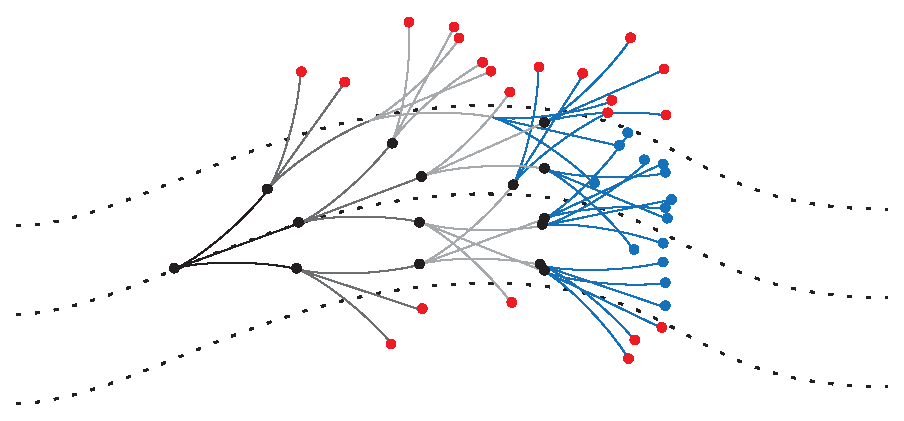
\includegraphics[width = \linewidth]{./_imags/Graph}
			\caption{Example graph. Visited nodes in black, dead end nodes in red, and non-visited nodes in blue.}
			\label {fig:Graph}
		\end{figure}
		It is worth stressing that you will be given both the %
		$\texttt{nodes}$ %
		and %
		$\texttt{edges}$ %
		arrays and you will not be involved in calculating their elements. %
		%
	\paragraph{Obstacles}
		To make the problem slightly more interesting, we consider not only path tracking but also collision avoidance.
		In particular, we would have to consider a set %
		$\mathcal{O} = \lbrace o_1, o_2, \cdots, o_{n_{obs}}\rbrace$, %
		of static obstacles to avoid, where each %
		$o_i\in\mathbb{R}^2$ %
		contains the position information of the obstacle %
		$i$.
	\paragraph{Node costs}
		In this exercise, we calculate the cost %
		$c_k$ %
		of a node %
		$k$ %
		as
		%
		\begin{align}
			c_k = c_j + c_{k,\text{path tracking}} + c_{k,\text{collision avoidance}} + c_{k,\text{dead end}}
		\end{align}
		%
		where 
		\begin{itemize}
			\item $c_j$ is the cost of the predecessor node, 
			\item $c_{k,\text{path-tracking}} = w_{\text{track-d}}x_2^2 + w_{\text{track-heading}}x_3^2$ %
			is a cost term associated with the path tracking error,
			\item $c_{k,\text{collision-avoidance}} = \sum_i^{n_{obs}} \frac{w_{collision-avoidance}}{dist(x_k, o_i)^2}$ %
			is a cost term associated with the proximity of a node to some specific obstacles, 
			\item $c_{k,\text{dead-end}} = \infty$ if $\gamma_k = 2$ %
			and %
			$c_{k,\text{dead-end}} = 0$ %
			otherwise. 
			This cost term prunes dead-end nodes of the solution.
		\end{itemize}
	\paragraph{Backtracking}	
		Once the graph is built and the cost of each node is assigned, the optimal trajectory is backtracked. 
		In particular, we first need to identify the set %
		$\mathcal{N}_T = \lbrace i : \gamma_k = 0\rbrace$ %
		of terminal nodes.
		Then, we select the one with the smallest cost %
		$i^* = \arg\min\lbrace c_i : i\in\mathcal{N}_T\rbrace$. %
		We later use the information in \texttt{edges} to explore the graph from %
		$i^*$ %
		in a backward manner by keeping track of the visited nodes, as they will be part of the optimal trajectory. 
 	%
\section{Provided files}
\begin{itemize}
	\setlength\itemsep{0em}
	\provFile{ex3.m}{The class whose methods have to be completed. 
		A brief description of its functions is provided within this document, whereas more detailed information regarding inputs and outputs can be found in the Matlab file itself.}
	\provFile{exercise3\_DynamicProgramming.m}{The Matlab script that sets up and runs the required simulations. 
		Even though, you are not asked to modify this script, understanding what the file does can be helpful to solve the problem.
		}
	\provFile{utilities.m}{The class which includes auxiliary functions.
		This file is updated w.r.t the one provided in previous exercises, and some bugs are fixed. 
		}
	\provFile{circle, path\_1, path\_2, path\_3} mat files contain different paths to be tracked which can be used in the experiments.		
\end{itemize}
%
\section{Exercises}
	\begin{itemize}
		\item Copy your solutions of the methods \texttt{getInitialState}, \texttt{getSystemParameters}, \newline and \texttt{select\_reference\_path} from previous exercises. 
		\item Complete the method \texttt{getAllowedControlValues} which returns an array including all possible combinations of control inputs that can be applied to the system. 
		Start by setting %
		$u_1 = 3$ %
		and %
		$u_2 \in \lbrace -\pi/4, 0, \pi/4 \rbrace$.
		\item Complete the method \texttt{getObstacle} which specifies the positions of the obstacles to be considered. You can start by positioning the obstacle(s) in an arbitrary location, and once you  visualize the path to be tracked, you can refine the position of the obstacle so that it is on the vehicle's way. 
		\item Complete the method \texttt{assignCostsToNodes} which explores the graph in a forward fashion from the initial node. This method assigns costs to the nodes. 
			You can freely choose the values of the weights corresponding to the cost function, but the values you report must result in collision-free trajectories. 
			If you cannot find such a set of parameters, explain why. 
		\item Complete the method \texttt{backtrackNodeValues} which explores the graph in a backward manner to collect the sequence of the nodes which define the optimal trajectory. 
		\item Repeat the exercise for different sets of obstacles (changing the number of obstacles and their position). 
		Is the algorithm always able to find a collision-free path? Why? 
		\item Why is the graph creation process randomized from a certain point on?
		\item If you obtained unexpected results, discuss them. 
	\end{itemize}
